\chapter{Containerization with Docker}
\label{cha:containerization-docker}
Docker is a tool for creating, provisioning and interacting with Linux Containers (LXC) \cite{Docker2018,LXC2018}. LXC are a lightweight version of virtualization, which does not have the resource impact of a full virtualization such as Operating System (OS) virtualization. The differences of LXC and a Virtual Machine (VM) are covered in Section \ref{sec:docker-virtualization-vs-containerization}. Docker has become very popular over the past years, due to the fact, that it made it possible to easily work with LXC. Docker relies strongly on the principles of IaC which has been discussed in Chapter \ref{cha:iac}. When using Docker, Linux Containers are often referred to as Docker Containers. \\

Containerization is a key factor when hosting applications in the cloud, because the applications are normally packaged in images and run as containers on the cloud platform. Containerization provides features for a fast, effortless and consistent way of running applications in the cloud, which is discussed in the following Section \ref{sec:docker-need-for-containerization}.

\section{The need for Containerization}
\label{sec:docker-need-for-containerization}
Containerization is a key factor for cloud platforms such as PaaS, where each application runs in its own isolated environment, called a container. A container is an instance of an image, which represents the initial state of an application. A VM represents a full blown OS, where the OS provides a kernel, which is emulated on the host OS by the Hypervisor. A Hypervisor is a software which can create, run and manage VMs. A container uses the kernel provided by the host OS and therefore there is no need for an emulation. A container does not represent a full blown OS, but still provides features normally provided by an OS such a networking and storage \cite{DockerVirtScheepers2014}. \\ 

Containers are faster to create, to deploy and easier to manage compared to VMs. Nevertheless, cloud platforms use virtualization for managing their infrastructure, where the containers run on the provisioned VMs. The usage of containers compared to the usage of VMs can reduce costs for hosting applications. Enterprises can profit from hosting their applications of containers in several ways. Applications hosted in containers need lees resources than applications hosted in VMs, because there is no virtualized OS and no need for kernel emulation. The creation, deployment and startup of containers are faster, because only the isolated process needs to be started and not a full blown OS. Docker is well supported by Integrated Development Environments (IDEs), which provide support for creating Docker Image definitions (Dockerfiles) and provisioning of Docker Containers on a local or remote environment \cite{DockerFile2018}. \\

When enterprises have applied IaC to their infrastructure, then the next logical step is to integrate their applications into IaC as well. Applications hosted in containers profit from the IaC principles immutability, reproducibility, repeatability and consistency. Therefore, Docker strongly relies on IaC and provides tooling for automating creation and provisioning of Docker Containers, which is used by PaaS platforms such as Openshift. With Docker, developers define the hosting environment for their applications and not system administrators anymore. Nevertheless, developers can profit from the deep Linux knowledge of system administrators, to define the Docker Images efficiently, to keep them small and secure. The following Section \ref{sec:docker} will give an overview of the Docker technology, its architecture and artifacts.  

\section{Docker}
\label{sec:docker}
This section covers Docker, which is the most popular tool to work with LXC. Docker is open source but also provides an enterprise support. The core part of the Docker technology is the Docker Engine, which is discussed in Section \ref{sec:docker-engine}. The Docker Engine is the part of the Docker technology that actually runs the containers. The Docker Images are managed in a so called Docker Registry, which is a repository for Docker Images. The most popular Docker Registry is Docker Hub, which is a free service, where anyone can provides Docker Images \cite{DockerRegistry2018}.

\subsection{Docker Engine}
\label{sec:docker-engine}
Figure \ref{fig:docker-engine} illustrates the Docker Engine architecture hosted on a Linux OS. The Docker Engine is build by layers, where each layer communicates with the layer beneath.

\begin{figure}[htbp]
	\centering
	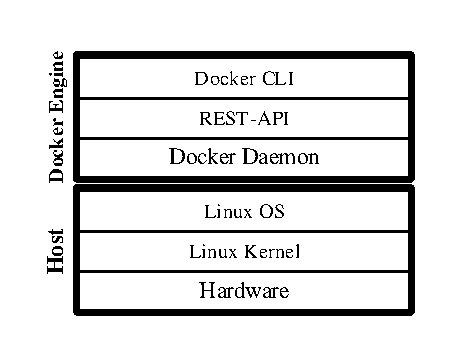
\includegraphics[scale=0.8]{images/docker-engine.pdf}
	\caption{Docker Engine architecture}
	\label{fig:docker-engine}
\end{figure} 

The Docker Engine was initially designed for LXC exclusively but has been ported to Windows. Docker Images and Containers created for Windows OS are not supported on a Linux OS and visa versa. The Docker Images and Containers for a Windows OS differ from those for a Linux OS, but the principles of Docker Images and Docker Containers are the same.

\mysubsubsection{Docker Damon}
\label{sec:docker-daemon}
The Docker Daemon represents the background process, which creates, runs and manages the Docker Containers on the Docker Host, similar to a VM Hypervisor. The Docker Daemon strongly depends on the kernel of the host OS, therefore incompatibilities could cause the Docker Daemon to fail functioning. The communication with the Docker Daemon is performed via a REST-API, because the Docker Engine is designed as a server client architecture. \\

\mysubsubsection{REST-API}
\label{sec:docker-rest-api}
The REST-API can be exposed via a Unix socket or a network interface, depending on the configuration of the Docker Daemon. If the REST-API is exposed via a network interface, then it is recommended to secure the connection with client certificate authentication. If the Docker Engine and the Docker Client are located on the same host, then commonly the REST-API is exposed via a Unix socket and does not need any special security. \\

\mysubsubsection{Docker Command Line interface}
\label{sec:docker-cli}
The Docker Engine provides a Docker Command Line Interface (CLI) for interacting with the Docker Daemon via a Linux shell. The Docker CLI itself communicates with the Docker Daemon via the exposed REST-API. This is the most common way to interact with a Docker Daemon. The Docker CLI provides commands for creating Docker Images and Containers and for provisioning the Docker Containers on the Docker Host. \\

\mysubsubsection{Docker Images}
\label{sec:docker-images}
Docker Images are defined via Dockerfiles, which contain instructions how to build the Docker Image. A Docker Image consists of layers, where each layer represents a state of the file system, produced by a Dockerfile instruction. Each layer is immutable and any change on the file system produces a new layer. Docker Images are hierarchical and can inherit from another Docker Image, which is then called base image. Docker Images support only single inheritance and the base image is defined via the \mentionedtext{FROM} instruction as the first instruction in the Dockerfile. Docker Image names have the structure \mentionedtext{[namespace]/[name]:[version]} e.g. \mentionedtext{library/openjdk:8-alpine}. \\

\mysubsubsection{Docker Containers}
\label{sec:docker-containers}
A Docker Container is an instance of a Docker Image, where a new layer is appended, which contains all changes made on the file system by the running process within the Docker Container. When the Docker Container is deleted, then the appended layer gets deleted as well and all made changes on the file system are lost. A Docker Container keeps running as long as the contained foreground process is running. Without a foreground process the Docker Container stops immediately after it was started. The process running in the Docker Container is isolated from other processes, as well is the file system, the process has access to. \\

\subsection{Docker Architecture}
\label{sec:docker-architecture}
The Figure \vref{fig:docker-architecture} illustrates the Docker architecture, which is a client server architecture. The design as a client server architecture is the reason why the communication to the Docker Daemon is performed via the provided REST-API. The Docker Client communicates with the Docker Daemon via the Docker CLI, where the Docker Client can be located on a remote host or on the Docker Host. The Docker Host hosts the Docker Engine, which exposes the REST-API the Docker Client connects to. The Docker Engine managed the Docker Images and Containers located on the Docker Host. The Docker Engine can pull Docker Images from a remote Docker Registry, if a registry has been registered.

\begin{figure}[htbp]
	\centering
	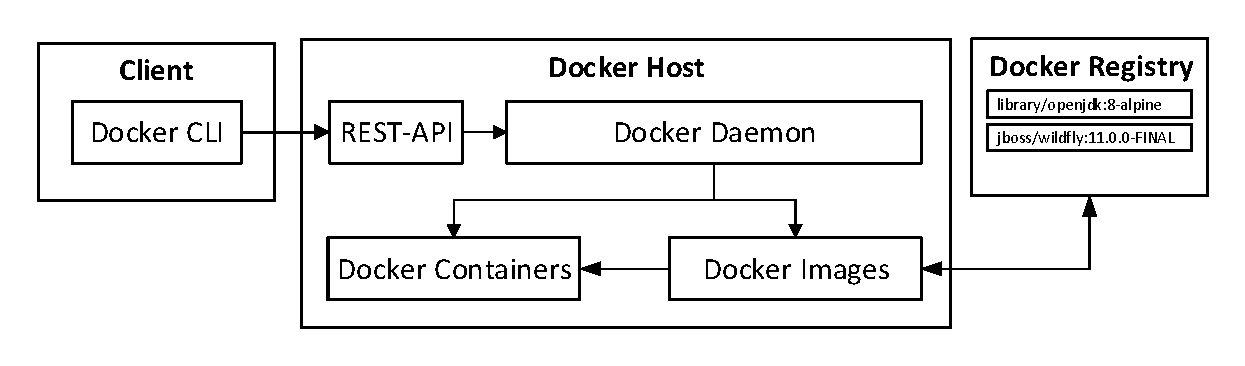
\includegraphics[scale=0.9]{images/docker-architecture.pdf}
	\caption{Docker Architecture}
	\label{fig:docker-architecture}
\end{figure} 

\subsection{Docker Machine}
\label{sec:docker-machine}
Docker Machine is a tool for managing local or remote Docker Hosts \cite{DockerMachine2018}. With Docker Machine an administrator can manage multiple Docker Hosts from a main server, without the need to connect to the Docker Host via secure shell (SSH). The Docker Machine CLI provides all commands necessary for managing Docker Hosts. Docker Engine provisions Docker Containers on a Docker Host and Docker Machine provisions Docker Hosts, in particular Docker Engines installed on docker Hosts. With Docker Machines a network of Docker Hosts can be managed, which is used by cloud platforms such as Openshift to manage Docker Engines on the nodes within the Openshift cluster.  

\section{Virtualization vs. Containerization}
\label{sec:docker-virtualization-vs-containerization}
Before LXC the industry made heavy use of operating system (OS) virtualization to isolate their environments and applications. A VM is managed by a Hypervisor, which is software, which can create, run and manage VMs. The VM provides resources such as network and storage for the application, which is managed by the virtualized OS. Nevertheless, an VM represents a full blown OS, which itself has a resource need which adds to the resource needs of the hosted application. LXC on the other hand are a kernel technology, which provides resources such as network and storage to the application as well, but without the need of virtualized OS.

\subsection{Virtual Machines}
\label{sec:docker-virtual-machines}
A Virtual Machine is an instance of a Virtual Machine Image (VMI), which is managed by a Virtual Machine Monitor (VMM), which is also referred to as the Hypervisor. The actual difference between a VMM and a Hypervisor is where the software is installed on. If the software is directly installed on the Hardware, then the software is called a Hypervisor, if its installed on the Host OS then its called a VMM. The VM abstracts  an Guest OS from the Host OS, in particular from the underlying hardware. A VM contained Guest OS is not bound to the underlying hardware, because the Hypervisor performs a kernel emulation, which allows to virtualize any Guest OS on any hardware, if the hypervisor supports it. The following Figure \ref{fig:docker-virtualization-architecture} illustrates the architecture of a virtualization system.

\begin{figure}[htbp]
	\centering
	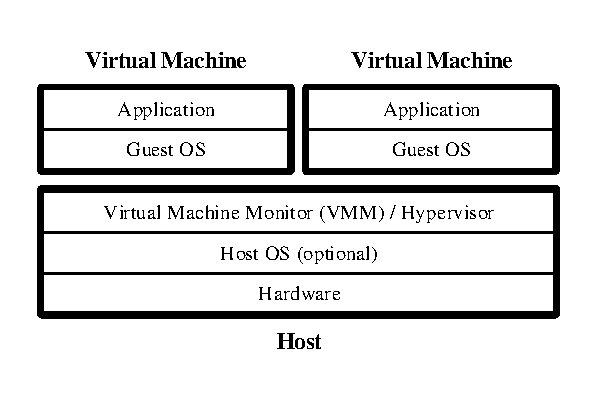
\includegraphics[scale=0.8]{images/docker-virtualization-architecture.pdf}
	\caption{Architecture of virtualized applications}
	\label{fig:docker-virtualization-architecture}
\end{figure} 

Glauber Costa's started the abstract of his talk at the LinuxCon 2012 with the humorous note \mentionedtext{"I once heard that Hypervisors are the living proof of operating system's incompetence"}. With this note he expressed that OS weren't able to provide proper isolation for applications and therefore the industry started to provide an OS instance for each application \cite{LxConCosta2012}. This has been overcome with the upcoming of LXC, which provide the proper isolation of applications on the same OS, which made the need for an OS instance for each application obsolete.

\subsection{Linux Container}
\label{sec:docker-linux-container}
The upcoming of LXC has eliminated the shortcoming to not be able to isolate applications properly of the Linux OS, which lead to using OS virtualization to isolate applications. LXC provide the feature of isolating applications running on the same OS, without the need of a kernel and hardware emulation as it is done with OS virtualization. As illustrated in Figure \ref{fig:docker-container-architecture}, the application process, binaries and libraries are bundled into the container and are isolated from other containers. Each container gets a portion o the global resources such as CPU cycles and memory assigned and cannot consume more as it has been assigned to. Without LXC it is possible that one process takes over the system resources and other processes get into state of starvation, which lead to need of OS virtualization. 

\begin{figure}[htbp]
	\centering
	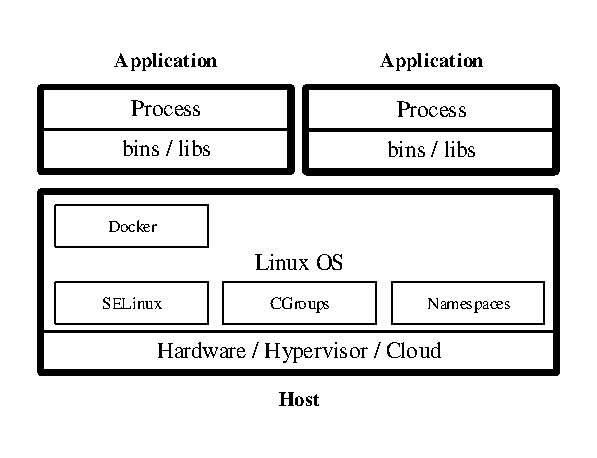
\includegraphics[scale=0.8]{images/docker-containerized-architecture.pdf}
	\caption{Architecture of containerized applications}
	\label{fig:docker-container-architecture}
\end{figure} 

The two main technologies underlying LXC are \mentionedtext{CGroups} and \mentionedtext{Namespaces}. These two kernel technologies provide the features needed for application isolation and prevention of process starvation.

\mysubsubsection{CGroups}
CGroups stands for control groups and CGroups provide the ability to aggregate processes, their child processes and threads within theses processes to groups managed in a tree structure. Each group gets a portion of the global resources such as CPU time, memory, I/O and network assigned, where its guaranteed that a group and its managed processes cannot consume more resources as the group has been assigned to. Each application hosted in a container is assigned to a group, where an application cannot steal resources from another application anymore, because the resource assignments of an group managed by CGroups prevents this from happening \cite{KernelCGroupsV12018, KernelCGroupV22015, IntelLXCHyperVisor2014}. \\

\mysubsubsection{Namepsaces}
CGroups manage how many resources can be used by group and namespaces manage the view of the system to a group. A container is managed in a namespace and therefore has a limited view of the system such as networks or other processes. Namespaces provide the isolation of a container.


